For each subject and phase (SA and FA) we hereby present a performance
result both for classification and regression. For classification, the
performance index is the percentage of correctly guessed labels, i.e.,
the amount of time during which the system is correctly predicting the
grasp the subject is applying (no grasp, index precision grip, other
fingers precision grip and power grasp). For regression, the
performance index is the correlation coefficient evaluated between the
predicted force signal and the real one. The choice of the correlation
coefficient, as opposed to the more standard Mean-Square Error, is
suggested by a practical consideration: when driving a prosthesis, or
even a non-prosthetic mechanical hand, we are not interested in the
absolute force values desired by the user/subject, since mechanical
hands usually cannot apply as much force as human hands do, for
obvious safety reasons. We are rather concerned in getting a signal
which is \emph{strongly correlated} with the user/subject's will.

As is standard in machine learning, each data set was split in $5$
folds and cross-validation was performed on it; this makes the
evaluation robust against the problem of over-fitting. We employed a
well-known freely available SVM package, \emph{libsvm} v2.83
\cite{ChangL01}, in the Matlab wrapped flavour, with a Gaussian
kernel. This particular kind of SVM requires setting two parameters,
called $\sigma$ and $C$, which were found by grid search using the
aforementioned performance indexes.

With respect to the previous Section, after an initial round of
experiments the values of $T_{RMS}$ and $d$ were set to:

\begin{itemize}

  \item $T_{RMS}=0.5s$ for classification, and $T_{RMS}=0.1s$ for regression;

  \item $d=0.02$ for the SA phase, and $d=0.032$ for the FA phase.

\end{itemize}

Classification proved to be more sensitive to high-frequency noise
than regression, and therefore we set a larger value of $T_{RMS}$ for
it; it is expected, anyway, that a delay of $500ms$ would be
compensated by the anticipatory nature of the EMG signal. This should
not, then, hinder the performance of the system in a practical
setting. As far as the value of $d$ is concerned, a slightly larger
value in the FA phase \textbf{BOH, Che ci scrivo?}

Figure \ref{fig:results} shows the main results obtained by the SVMs.

\begin{figure*}[!ht] \centering
  \begin{tabular}{cc}
    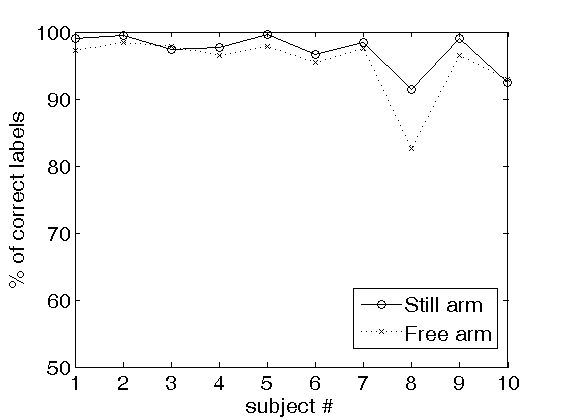
\includegraphics[width=0.45\textwidth]{figs/perfClass} &
    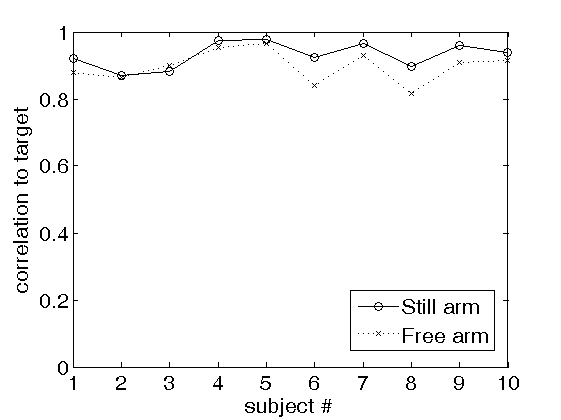
\includegraphics[width=0.45\textwidth]{figs/perfRegr} \\
    $(a)$ & $(b)$ \\
  \end{tabular}
  \caption{classification $(a)$ and regression $(b)$ results obtained
    by the system, on both phases of the experiment (FA and SA) and
    for each subject.}
  \label{fig:results}
\end{figure*}

Consider the Figure, panel $(a)$, showing the classification
performance. It is clear that the system attains an excellent accuracy
overall, namely $95.74\% \pm 3.76\%$ in the SA phase, and $93.76\% \pm
4.32\%$ in the FA phase. The worst result is obtained by subject $8$,
$87.73\%$ in SA and $82.80\%$ in FA. Moreover, the performance is
consistent by subject and by phase, meaning that $(a)$ hard subjects
in the SA phase are hard as well in the FA phase and viceversa, and
$(b)$ the FA phase is always harder than the SA phase. Since the
duration of the two phases (and consequently the numebr of samples
available to the system) is roughly the same less controlled
conditions make the problem harder, as one would expect.

Consider now panel $(b)$ of the same Figure, showing the regression
performance: here the performance is good to excellent, being $0.83
\pm 0.1$ for the SA phase and $0.72 \pm 0.13$ for the FA phase. The
hardness pattern seen in classification is repeated almost perfectly,
the FA phase being harder than the SA phase consistently by
subject. Remarkably, not all subjects which are hard for regression
(namely, $1,2,3,6,8$) happen to be hard for classification; in
particular, only subject $8$ is definitely hard \emph{both} for
classification and regression, while, e.g., subject $1$ obtains bad
results in both. This fact is indeed \emph{not} due to the number of
samples in the training set, since $1$ has $783/2308$ samples
(classification/regression) and $8$ has $1092/3133$, that is, roughly
the same proportion. This indicates that subject $1$ obtains a good
result in classification with about one-third of the samples used for
regression, whereas subject $8$ cannot do the same. Moreover, subject
$8$ happens to have \emph{more} samples available for classification
($1092$) than subject $1$ ($783$), and nevertheless obtains a much
worse performance.



